\documentclass{beamer}

\beamertemplatenavigationsymbolsempty
\setbeamerfont{page number in head/foot}{size=\small}
\setbeamertemplate{footline}[frame number]
\usefonttheme[onlymath]{serif}

\usepackage[utf8]{inputenc}

\usepackage[T1]{fontenc}
\usepackage[english]{babel}
%\usepackage[utf8]{inputenc}

\usepackage{tikz}
\usetikzlibrary{calc}
\usetikzlibrary{arrows, backgrounds}
\usetikzlibrary{matrix, arrows.meta}
\usetikzlibrary{decorations.pathreplacing}

% Scale all pgf plots, not only coordinates
\usepackage{adjustbox}

%\usepackage{amsfonts}
%\usepackage{amsmath}
%\usepackage{amsthm}
\usepackage{bm}

\usepackage{pgfplots}
\pgfplotsset{compat=1.3}
\usepgfplotslibrary{groupplots}

% Used for split environment
\usepackage{amsmath}
% Separate rows in align environment by this amount
\addtolength{\jot}{1em}

\usepackage{graphicx}
\graphicspath{{../fig/} {fig/}}
\usepackage{subfig}
\usepackage{wrapfig}

% Clickable links
\usepackage{hyperref}
\hypersetup{
	colorlinks,
	citecolor=black,
	filecolor=black,
	linkcolor=black,
	urlcolor=black
}

\usepackage[pdf]{graphviz}

%\usepackage[dvipsnames]{xcolor}
\usepackage{listings}

\lstset{
	language=c,
  basicstyle=\small\ttfamily,  % the size of the fonts that are used for the code
	numbers=none,                   % where to put the line-numbers
  inputencoding=latin1,
  numberstyle=\tiny,  % the style that is used for the line-numbers
  stepnumber=1,                   % the step between two line-numbers. If it's
				    %1, each line 
                                  % will be numbered
  %numbersep=5pt,                  % how far the line-numbers are from the code
  backgroundcolor=\color{white},      % choose the background color.
  showspaces=false,               % show spaces adding particular underscores
  showstringspaces=false,         % underline spaces within strings
  showtabs=false,      % show tabs within strings adding particular underscores
	frame=none,                   % adds a frame around the code
  rulecolor=\color{black},        % if not set, the frame-color may be changed
				   % on line-breaks within not-black text (e.g.
				   % comments (green here))
	tabsize=6,                      % sets default tabsize to 2 spaces
  columns=fullflexible,
  extendedchars=true,
  captionpos=b,                   % sets the caption-position to bottom
  breaklines=true,                % sets automatic line breaking
  breakatwhitespace=false,        % sets if automatic breaks should only happen
				    %at whitespace
  title=\lstname,                   % show the filename of files included with
				    %\lstinputlisting;
                                  % also try caption instead of title
  keywordstyle=\color{blue},          % keyword style
	commentstyle=\color{gray},       % comment style
	stringstyle=\color{brown},         % string literal style
  escapeinside={\%*}{*)},            % if you want to add LaTeX within your code
	morecomment=[l][\color{purple}]{\#},
	moredelim=[il][\color{purple}]{@},
%	abovecaptionskip=-15pt
%	belowcaptionskip=-15pt
}


\usepackage{csquotes}

\usepackage{siunitx}

\usepackage{multicol}

\usepackage{epigraph}
\setlength{\epigraphwidth}{0.7\textwidth}

\usepackage{caption}
\captionsetup{font=footnotesize}

% Macros para ayudar a la redacción
% Vector
\newcommand*\mat[1]{ \begin{pmatrix} #1 \end{pmatrix}}
\newcommand*\arr[1]{ \begin{bmatrix} #1 \end{bmatrix}}
\newcommand*\V[1]{\bm{#1}}
\newcommand{\E}{\V{E}}
\newcommand{\rhog}{\rho_\text{ghost}}
\newcommand{\F}{\V{F}}
\newcommand{\B}{\V{B}}
\renewcommand*{\v}{\V{v}}
\newcommand{\x}{\V{x}}
\newcommand{\dt}{\Delta t}
\newcommand{\dx}{\Delta x}
\newcommand*\neigh[1]{\mathcal{N}(#1)}

% Norm
\newcommand\norm[1]{\left\lVert#1\right\rVert}

\title{Particle-in-cell plasma simulation with OmpSs-2}
\author{Rodrigo Arias Mallo}
\date{\today}

\begin{document}

\frame{\titlepage}

\begin{frame}
\frametitle{Outline}
\tableofcontents
\end{frame}

\section{Introduction}

\begin{frame}{Introduction}
What exactly is a plasma?

Talk about 2D only.

Introduce species.

Plasma must be neutral.

\end{frame}

\begin{frame}{Introduction}
A plasma is an almost neutral gas of charged and neutral particles which 
exhibits collective behavior.

\vspace{1em}
Simulation can provide insight in the behavior of plasma without expensive 
laboratory equipment.
\end{frame}

\section{Model}

\begin{frame}{Vlaslov equation}
The Vlaslov equation describes the evolution of a plasma, with long range 
iteration between particles.
\begin{equation}%{{{
\frac {\partial f_j}{\partial t} +
\v \cdot \frac {\partial f_j}{\partial \V x } +
\frac{q_j}{m_j} \left( \E + \frac{\v \times \B}{c} \right) \cdot
	\frac {\partial f_j}{\partial \V v}
=0
\end{equation}%}}}
Where $f_j(\x,\v,t)$ is the distribution function of the specie $j$, and the 
fields electric $\E$ and magnetic $\B$ are determined by Maxwell equations.
\end{frame}

\begin{frame}{Maxwell equations}{}
The evolution of the fields is governed by the Maxwell equations
\small
\begin{align}%{{{
\begin{split}
\nabla \cdot \E &= \frac {\rho }{\epsilon_0} \\
\nabla \cdot \B &= 0 \\
\end{split}
&
\begin{split}
\nabla \times \E &= - \frac {\partial \B }{\partial t} \\
\nabla \times \B &= \mu_0 \left(\V J +
	\epsilon_0 \frac{\partial \E}{\partial t}\right) \\
\end{split}
\end{align}%}}}
%
\normalsize
Where $\rho$ is the charge density distribution, $\V J$ the current field and
$\epsilon_0$ and $\mu_0$ are constants.

\end{frame}


\begin{frame}{Electrostatic approximation}{}
In our model, we will only have a \textbf{strong fixed magnetic field} $\B_0$ 
and the Maxwell equations can be simplified.
\small
\begin{align}%{{{
\begin{split}
\nabla \cdot \E &= \frac {\rho }{\epsilon_0} \\
\end{split}
&
\begin{split}
\nabla \times \E &= 0 \\
\end{split}
\end{align}%}}}
\normalsize
\pause
As the electric field is irrotational, we can introduce a scalar field $\phi$, 
the electric potential, and rewrite $\E$ as a gradient $\E = - \nabla \phi$.  
Finally, if we solve for $\phi$ we obtain the Poisson equation:
\begin{equation}%{{{
\nabla^2 \phi = - \frac{\rho}{\epsilon_0},
\end{equation}%}}}
This approximation is called \textbf{electrostatic} as opposed to the 
\textbf{electromagnetic} case, when $\B$ varies with time.
\end{frame}

%\section{Discrete model}

\begin{frame}{The particle-in-cell method}{}
Solving the Vlaslov equation directly is very \textbf{computationally 
expensive}. The current solution is to introduce a spatial grid where the 
Maxwell equations are solved.

\vspace{1em}
The distribution function $f_j$ is then modeled by macro-particles which 
interact with the grid by an interpolation method.

\vspace{1em}
This method is known as \textbf{particle-in-cell} (PIC).
\end{frame}

\begin{frame}{The particle-in-cell method}{}
The space of length $\V L$ is discretized into grid points with a separation 
$\Delta \x$.

\vspace{1em}
The scalar fields $\rho$ and $\phi$ are now matrices of size $\V G = (G_x, G_y)$

\vspace{1em}
The vector field $\E$ is decomposed into $E_x$ and $E_y$, which are now matrices 
of the same size.

\end{frame}

\begin{frame}{The particle-in-cell method}{}

The PIC method has four main steps

\begin{itemize}
\setlength\itemsep{1em}
\item \textbf{Charge accumulation}: The charge density $\rho$ is interpolated in 
the grid from the particle positions.
\pause
\item \textbf{Solve field equation}: From the charge density the electric 
potential is obtained $\phi$ and then the electric field $\E$.
\pause
\item \textbf{Interpolation of electric field}: The electric field is  
interpolated back to the particle positions.
\pause
\item \textbf{Particle motion}: The force is computed from the electric field at 
the particle position and the particle is moved accordingly.
\end{itemize}
\end{frame}

\begin{frame}{Charge accumulation}{}

At each grid point $g$ at $\x$, the charge of each particle $p$ at $\x_p$ is 
accumulated using an interpolation function $W$.
\begin{equation}%{{{
\rho(\x) = \sum_p q\,W(\x - \x_p) + \rho_0
\label{eq:charge-accumulation}
\end{equation}%}}}
Using linear interpolation, we can define $W$ for two dimensions as
\begin{equation}%{{{
W(\x) =
\begin{cases}
			\displaystyle\left(1 - \frac{|x|}{\Delta x}\right)
				\left(1 - \frac{|y|}{\Delta y}\right) & \text{if}\ -\Delta\x < \x < 
				\Delta \x\\
			0 & \text{otherwise}
\end{cases}
\end{equation}%}}}
\end{frame}


\begin{frame}{Charge accumulation}{}
\begin{figure}[]%{{{
\centering
\scalebox{0.7} {
\begin{tikzpicture}[
		>=latex,
		effect/.style={dashed,-{Latex[length=3mm, width=1mm]}},
		particle/.style={fill=black,radius=3pt},
	]
	\draw [step=2cm,dotted] (1,1) grid (5,5);
	\coordinate (p) at (2.5,3.2);
	\coordinate (center) at (3,3);
	\coordinate (A) at ($(center)+(-1,1)$);
	\coordinate (B) at ($(center)+(1,1)$);
	\coordinate (C) at ($(center)+(1,-1)$);
	\coordinate (D) at ($(center)+(-1,-1)$);
	\draw[effect] (p) -- (A);
	\draw[effect] (p) -- (B);
	\draw[effect] (p) -- (C);
	\draw[effect] (p) -- (D);
	\node[above left]  at (A) {$A$};
	\node[above right] at (B) {$B$};
	\node[below right] at (C) {$C$};
	\node[below left]  at (D) {$D$};
	\draw[particle] (p) circle;
	\node[left] at (p) {$p$};
\end{tikzpicture}
\hspace{0.5cm}
\begin{tikzpicture}[
		>=latex,
		box/.style={black},
		particle/.style={fill=black,radius=3pt},
		div/.style={dashed},
	]
	\draw [step=2cm,dotted] (1,1) grid (5,5);
	\coordinate (p) at (2.5,3.2);
	\coordinate (center) at (3,3);
	\coordinate (A) at ($(p)+(-1,1)$);
	\coordinate (B) at ($(p)+(1,1)$);
	\coordinate (C) at ($(p)+(1,-1)$);
	\coordinate (D) at ($(p)+(-1,-1)$);
	\draw[box] (A) -- (B) -- (C) -- (D) -- (A);
	\draw[div] ($(A)!(center)!(B)$) -- (center);
	\draw[div] ($(B)!(center)!(C)$) -- (center);
	\draw[div] ($(C)!(center)!(D)$) -- (center);
	\draw[div] ($(D)!(center)!(A)$) -- (center);
	\node at ($(center)!0.5!(A)$) {$a$};
	\node at ($(center)!0.5!(B)$) {$b$};
	\node at ($(center)!0.5!(C)$) {$c$};
	\node at ($(center)!0.5!(D)$) {$d$};
	\draw[particle] (p) circle;
\end{tikzpicture}
\hspace{0.5cm}
\begin{tikzpicture}[
		>=latex,
		box/.style={black},
		particle/.style={fill=black,radius=3pt},
		div/.style={dashed},
	]
	\draw [step=2cm,dotted] (1,1) grid (5,5);
	\coordinate (p) at (2.5,3.2);
	\coordinate (center) at (3,3);
	\coordinate (A) at ($(center)+(-1,1)$);
	\coordinate (B) at ($(center)+(1,1)$);
	\coordinate (C) at ($(center)+(1,-1)$);
	\coordinate (D) at ($(center)+(-1,-1)$);
	\draw[box] (A) -- (B) -- (C) -- (D) -- (A);
	\draw[div] ($(A)!(p)!(B)$) -- (p);
	\draw[div] ($(B)!(p)!(C)$) -- (p);
	\draw[div] ($(C)!(p)!(D)$) -- (p);
	\draw[div] ($(D)!(p)!(A)$) -- (p);
	\node at ($(p)!0.5!(A)$) {$c$};
	\node at ($(p)!0.5!(B)$) {$d$};
	\node at ($(p)!0.5!(C)$) {$a$};
	\node at ($(p)!0.5!(D)$) {$b$};
	\draw[particle] (p) circle;
\end{tikzpicture}
}
\caption{Interpolation of particle $p$ charge into the four grid points A to D.}
\label{fig:interpolation}
\end{figure}%}}}
\end{frame}

\begin{frame}{Field equations}{}
First the electric potential $\phi$ must be computed from $\rho$, and then the 
electric field $\E$.

\vspace{1em}
Several methods are available for solving the Poisson equation:

\begin{itemize}
\setlength\itemsep{1em}
\item \textbf{Iterative  methods}: Jacobi, Gauss-Seidel, Successive Over 
Relaxation (SOR), Chebyshev...
\item \textbf{Matrix methods} Thomas Tridiagonal algorithm, Conjugate-Gradient, 
LU, Incomplete Decomposition...
\item \textbf{Spectral methods} A family of methods that use the fast Fourier 
transform (FFT).
\end{itemize}

\vspace{1em}
We will only focus on two methods: The LU decomposition used as debug, and MFT, 
a spectral method with complexity $O(N_g \log N_g)$.
\end{frame}

\begin{frame}{LU solver}
The Poisson equation is transformed in a linear system of $N_g$ equations (one 
for each grid point).
\begin{equation}
\label{eq:eq-system}
\nabla^2 \phi = - \frac{\rho}{\epsilon_0}
\quad \rightarrow \quad
A\frac{\phi}{\Delta x ^2 \Delta y^2} = -\frac{\rho}{\epsilon_0}
\quad \rightarrow \quad
Ax = b
\end{equation}
The coefficient matrix $A$ has non-zero coefficients only at $a_{ii} = 4$ and 
$a_{ij} = -1$ with $j \in \{i+1, i-1, i+N_x, i-N_x\} \mod N_x$, for all $0 \le i 
\le Ng$.

\vspace{1em}
The decomposition $A = LU$ is used to form two systems of equations $Ux = u$ and 
$Ly=b$, with a computational cost of $O(N_g^3)$ (but only at the beginning), 
which are solved in each iteration with cost $O(N_g^2)$.
\end{frame}

\begin{frame}{MFT solver}
Let $g = $
\begin{center}%{{{
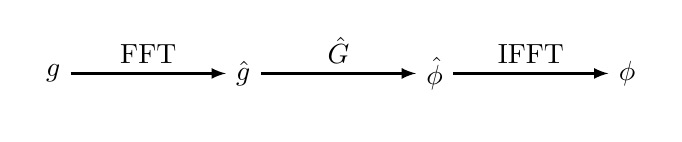
\begin{tikzpicture}[>=latex,thick,ampersand replacement=\&]
	\matrix (m) [
		matrix of nodes,
		column sep=20mm,
		nodes={
			%line width=1pt,
			anchor=center,
			text centered,
			%minimum width=1cm,
			minimum height=8mm,
		},
%		txt/.style={text width=1.5cm,anchor=center},
	]
	{
		$g$ \& $\hat g$ \& $\hat \phi$ \& $\phi$ \\
	};
	\foreach \i [evaluate={\j=int(\i+1)}] in {1,...,3}{
		\draw[->] (m-1-\i) -- (m-1-\j);
	}
	\draw[draw=none] (m-1-1) -- (m-1-2) node[midway,above] {FFT};
	\draw[draw=none] (m-1-2) -- (m-1-3) node[midway,above] {$\hat G$};
	\draw[draw=none] (m-1-3) -- (m-1-4) node[midway,above] {IFFT};
%	\draw[draw=none] (m-1-4) -- (m-1-5) node[midway,above]
%	{Eq.~\ref{eq:phi-to-E}};
\end{tikzpicture}
\end{center}%}}}
\end{frame}

\section{Sequential simulator}


\begin{frame}{Sequential simulator}{}
A sequential version of the simulator was produced to test the model with a 
visualization module to see the fields in real-time.

\vspace{1em}
Both simulations in 1D and 2D are supported.
\end{frame}
\begin{frame}{}{}
\begin{figure}[h]
	\centering
	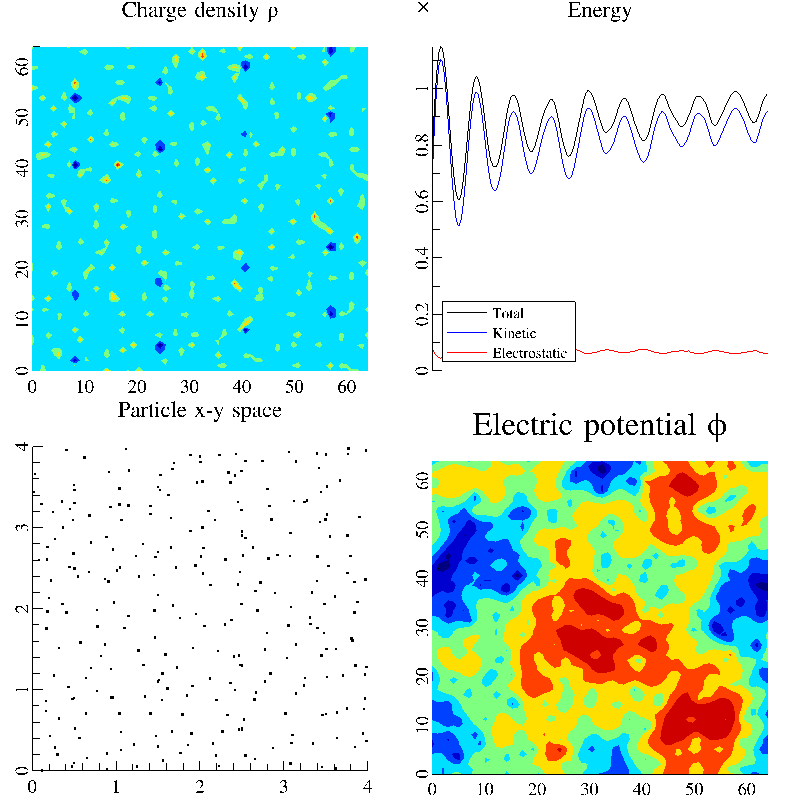
\includegraphics[height=0.95\textheight]{landau.png}
	\caption{Example run in 2D of the simulator in debug mode.}
	\label{fig:debug-mode}
\end{figure}
\end{frame}

\begin{frame}{Test: Conservation of energy}{}
\begin{figure}[h]
	\centering
	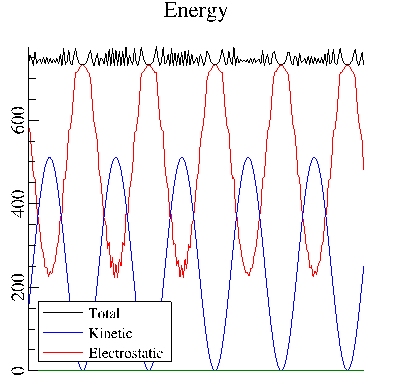
\includegraphics[width=0.4\linewidth]{1d-2particles-energy.png}
	\caption{Energy conservation in two particle test as shown in the simulator.}
	\label{fig:1d-2particles-energy}
\end{figure}
\end{frame}

\section{Parallel simulator}

\begin{frame}{Parallelization}
\begin{figure}[ht]%{{{
\centering
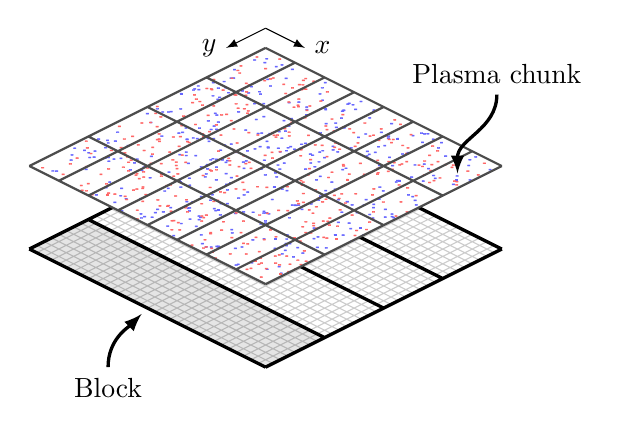
\begin{tikzpicture}[scale=0.5]
\begin{scope}[
		x=1cm,
		y=1cm,
		yshift=0,
		every node/.append style={
			yslant=0.5,xslant=-1},
		yslant=0.5,
		xslant=-1
	]
	% opacity to prevent graphical interference
	\draw[step=1.5/8, black!20!white, thin] (0,0) grid (6,6); %defining grids
	%\draw[step=1.5, black] (0,0) grid (6,6);
	\draw[xstep=1.5, ystep=6, black, very thick] (0,0) grid (6,6);
	%\draw[dashed, xstep=6, ystep=1.5, black] (0,0) grid (6,6);
	\fill[fill=black,fill opacity=0.1] (0,0) rectangle (1.5,6);
	\coordinate (a0) at (4.5, 0);
	\coordinate (a1) at (6, 0);
	\coordinate (a2) at (4.5, 1.5);
	\coordinate (a3) at (6, 1.5);

	\coordinate (b) at (0,3);

\end{scope}
\begin{scope}[
		x=1cm,
		y=1cm,
		yshift=60,
		every node/.append style={
			yslant=0.5,xslant=-1},
		yslant=0.5,
		xslant=-1
	]
	\coordinate (b0) at (4.5, 0);
	\coordinate (b1) at (6, 0);
	\coordinate (b2) at (4.5, 1.5);
	\coordinate (b3) at (6, 1.5);
	\coordinate (c) at (4.5+0.75, 0.75/2);
	%Idem as above, for the n-th grid:
%	\draw[dotted] (a0) -- (b0);
%	\draw[dotted] (a1) -- (b1);
%	\draw[dotted] (a2) -- (b2);
%	\draw[dotted] (a3) -- (b3);
%
%	\draw[dashed] (a2) -- (a3);

	\fill[fill=white,fill opacity=1.0] (0,0) rectangle (6,6);
	\begin{axis}[width=7.5cm,height=7.5cm,
						axis lines=none,
						%hide axis,
						xmin=-1, xmax=1,
						ymin=-1, ymax=1,
						inner frame sep=0,
				]
	\addplot [blue!60!white, only marks,
		mark=*, samples=400, mark size=0.75] (rand, rand);
	\addplot [red!60!white, only marks,
		mark=*, samples=400, mark size=0.75] (rand, rand);
	\end{axis}
	%\draw[step=1.5, black, thick] (0,0) grid (6,6);
	\draw[xstep=1.5, ystep=1.5/2, black!70!white, thick] (0,0) grid (6,6);
	%\draw[dashed,xstep=6, ystep=1.5, black, thick] (0,0) grid (6,6);


	\coordinate (O) at (6.5, 6.5);
\end{scope}

\draw[-latex,very thick] (c)+(1,2) node[above]{Plasma chunk}
				to[out=-90,in=90] (c);
\draw[-latex,very thick,shorten >=3pt] (b)+(-1,-1.5) node[below]{Block}
				to[out=90,in=180+45] (b);

\begin{scope}[
		y={(-1cm,0.5cm)},x={(1cm,0.5cm)}, z={(0cm,1cm)},
	]
%	\coordinate (O) at (-3, 3.5, 0);
%	\draw[-latex] (O) -- +(1, 0,  0) node [right] {$x$};
%	\draw[-latex] (O) -- +(0, -1, 0) node [right] {$y$};
%	\coordinate (O) at (-0.75, -0.75, 0);
	\draw[-latex] (O) -- +(-1, 0,  0) node [left] {$y$};
	\draw[-latex] (O) -- +(0, -1, 0) node [right] {$x$};
\end{scope}
\end{tikzpicture}
\caption{Domain decomposition: The plasma is divided into chunks in both 
directions and the fields into blocks in the Y dimension only}
\label{fig:domain-decomposition}
\end{figure}%}}}
\end{frame}



\section{Results}

\begin{frame}{Multithread FFT}

The FFTW library has a very bad performance with threads.

\begin{figure}[h]%{{{
	\centering
	\begin{adjustbox}{max totalsize={.7\textwidth}{.5\textheight},center}
		\begin{tikzpicture}
		\begin{axis} [
			legend pos=north west,
			xmode=log,
			log basis x=2,
			xticklabels={0,1,2,4,8,16,32},
			grid=major,
			xlabel=Number of CPUs,
			ylabel=Time per iteration (s),
			width=10cm,
			height=6cm,
			]
		\addplot+ [error bars/y dir=both, error bars/y explicit] table [
			x index = {0},
			y index = {3},
			y error index={4},
			col sep=space] {perf/fftw-sequential/time.csv};
		\addlegendentry{Single thread}
		\addplot+ [error bars/y dir=both, error bars/y explicit] table [
			x index = {0},
			y index = {3},
			y error index={4},
			col sep=space] {perf/fftw-threads/time.csv};
		\addlegendentry{Multithread}
		\end{axis}
		\end{tikzpicture}
		\end{adjustbox}
	\caption{The number of CPUs is increased with only one process: the solver 
	cannot scale and the time per iteration increases. Configuration used: $N_p = 
	\num{5e5}$, $N_g=8192\times8192$.}
	\label{fig:fftw-time}
\end{figure}%}}}
\end{frame}

\begin{frame}{Strong scaling with $N_g=2048^2$}
\begin{figure}[ht]%{{{
\centering
\begin{adjustbox}{max totalsize={.9\textwidth}{.7\textheight},center}
\begin{tikzpicture}
	\begin{axis}[
		xmode=log,
		log basis x=2,
		xticklabels={0,1,2,4,8,16,32},
		grid=major,
		xmin=0,
		ymin=0,
		xlabel=Number of nodes,
		ylabel=Speedup,
		height=8cm,
		width=0.7\textwidth,
		/tikz/font=\small]
		\addplot+ table [
			x = P,
			y = speedup,
			col sep=tab] {perf/strong-scaling-fixed/csv/time.csv};
	\end{axis}
\end{tikzpicture}
\begin{tikzpicture}
	\begin{axis}[
		xmode=log,
		log basis x=2,
		xticklabels={0,1,2,4,8,16,32},
		grid=major,
		xmin=0,
		ymin=0,
		xlabel=Number of nodes,
		ylabel=Efficiency,
		height=8cm,
		width=0.7\textwidth,
		/tikz/font=\small]
		\addplot+ table [
			x = P,
			y = efficiency,
			col sep=tab] {perf/strong-scaling-fixed/csv/time.csv};
	\end{axis}
\end{tikzpicture}
\end{adjustbox}
	\caption{Strong scaling with configuration: $N_p = \num{1e8}$, $N_g = 2048^2$,	
	$N_c = 128$, one process per node, using each 48 cores.}
	\label{fig:strong-scaling}
\end{figure}%}}}
\end{frame}
\section{Discussion}

\begin{frame}{End}
Thanks for your attention.
\end{frame}

\end{document}
